\section{Part 1 -- Architecture}

%Describe the model you created.
%Here you will describe the identified architecture, the chosen design decisions, the relevant information about the produced models, such as smart solutions applied, how you organized the architectural specification in a modular way, \etc

The primary goal of our AADL model was to specify components of the Smart Fire Alarm system with enough detail to provide a reasonable estimate of data transmission latency between relevant devices. To do this, we organized elements of the network into three layers: (1) the top layer, which describes three sub-networks; (2) the middle layer which describes the physical devices forming each sub-network; and (3) the bottom layer describing internal details of some of these devices.

The first layer is formed by three sub-networks. The Sensor Network contains devices connected using short-ranged wireless communication technologies (Wi-fi, Bluetooth and Zigbee) and, in a real-world implementation, would be placed within the same house or building. The Communication Network provides a very high-level abstraction of the infrastructure that allows the connection between two remote locations over the Internet. Finally, the Control Center is also a high-level abstraction of the location where sensor data is gathered for analysis and also where an alarm signal is received if it is necessary to dispatch emergency services.

\autoref{fig:smartfirealarm} shows a broad overview of the system and how the three sub-networks connect to each other. The Sensor Network connects to the Communication Network through two ports, depending on which communication technology is used, and data is then forwarded into the Control Center over a wired Internet connection.

%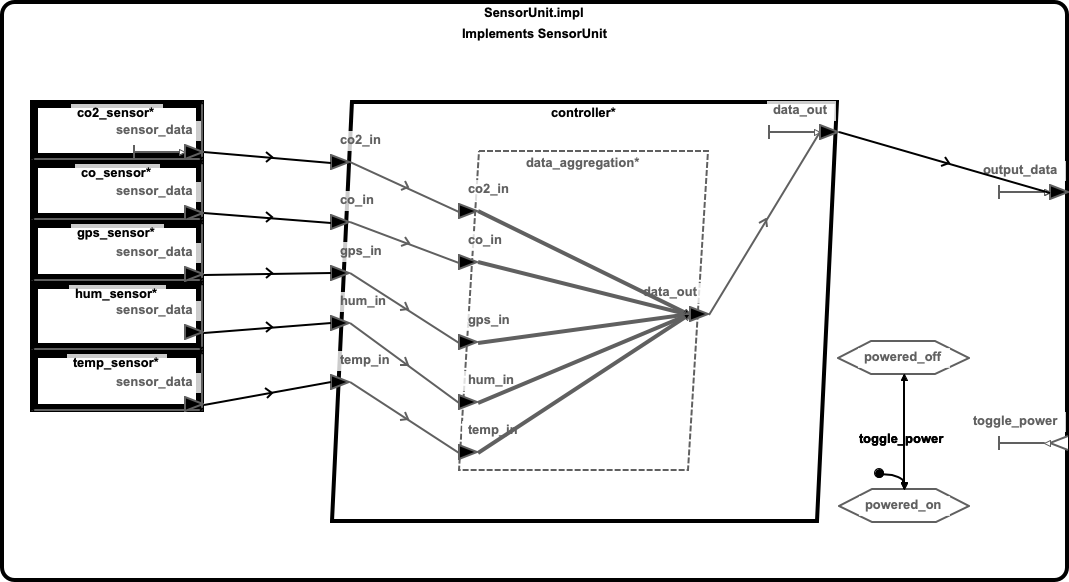
\includegraphics[width=\textwidth]{SensorUnit.png}

\begin{figure*}[h]
\caption{General structure of the system}
\label{fig:smartfirealarm}
\centering
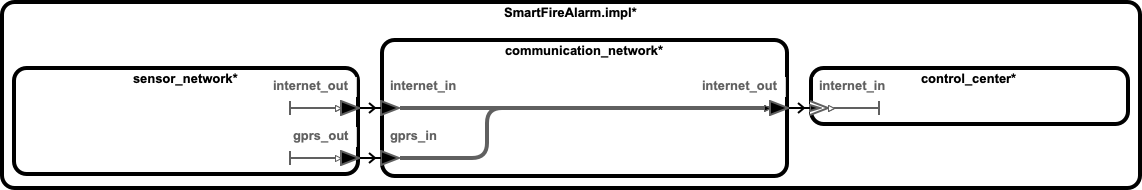
\includegraphics[width=0.9\textwidth]{SmartFireAlarm}
\end{figure*}

\begin{figure*}[h]
\caption{Structure of the Sensor Network}
\label{fig:sensornetwork}
\centering
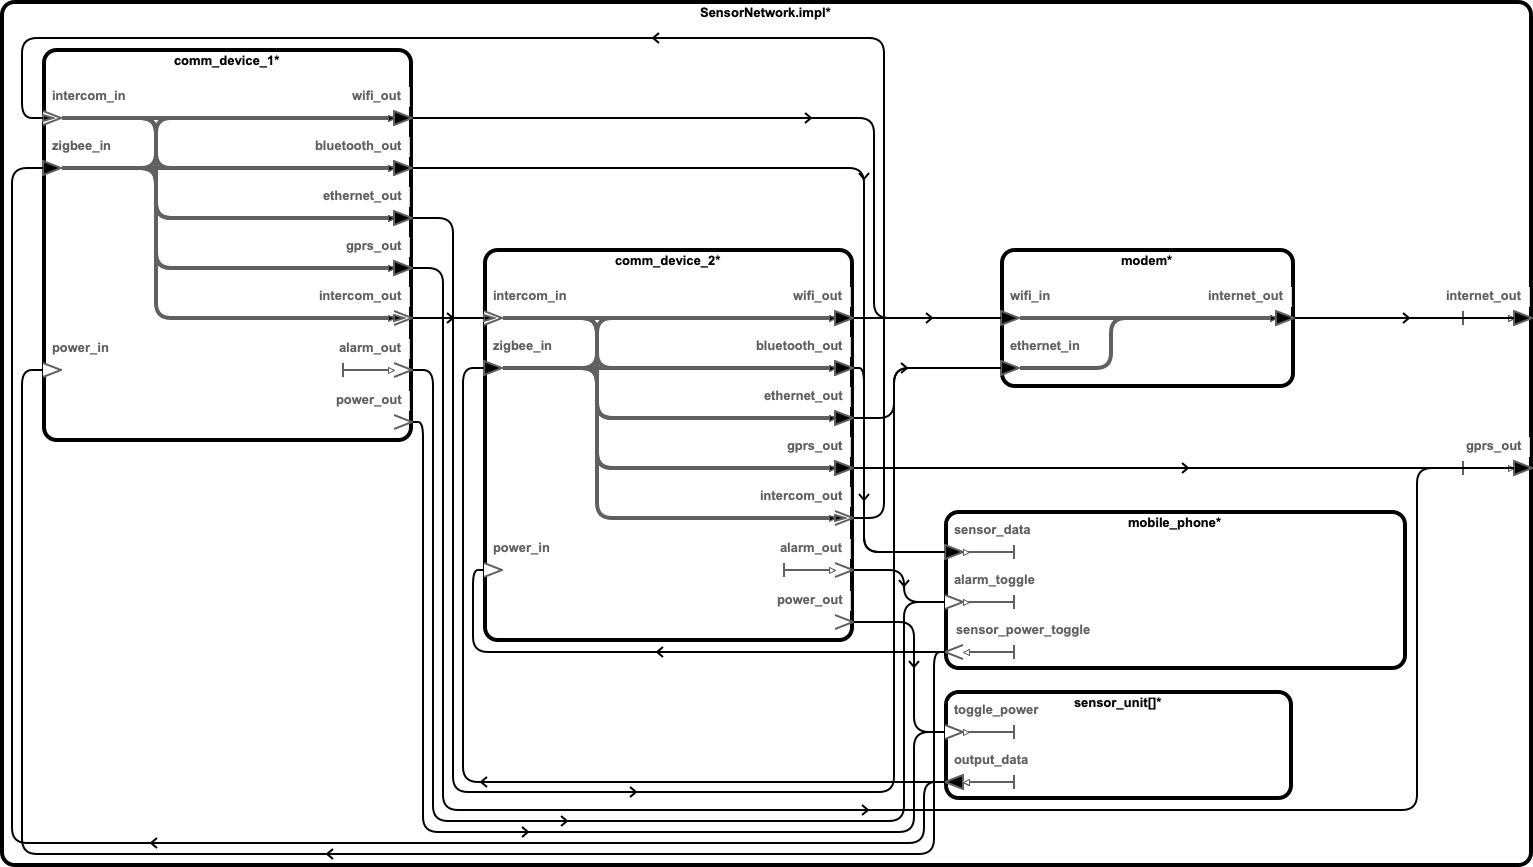
\includegraphics[width=0.9\textwidth]{SensorNetwork}
\end{figure*}

\begin{figure*}[h]
\caption{Internal structure of a Sensor Unit}
\label{fig:sensorunit}
\centering
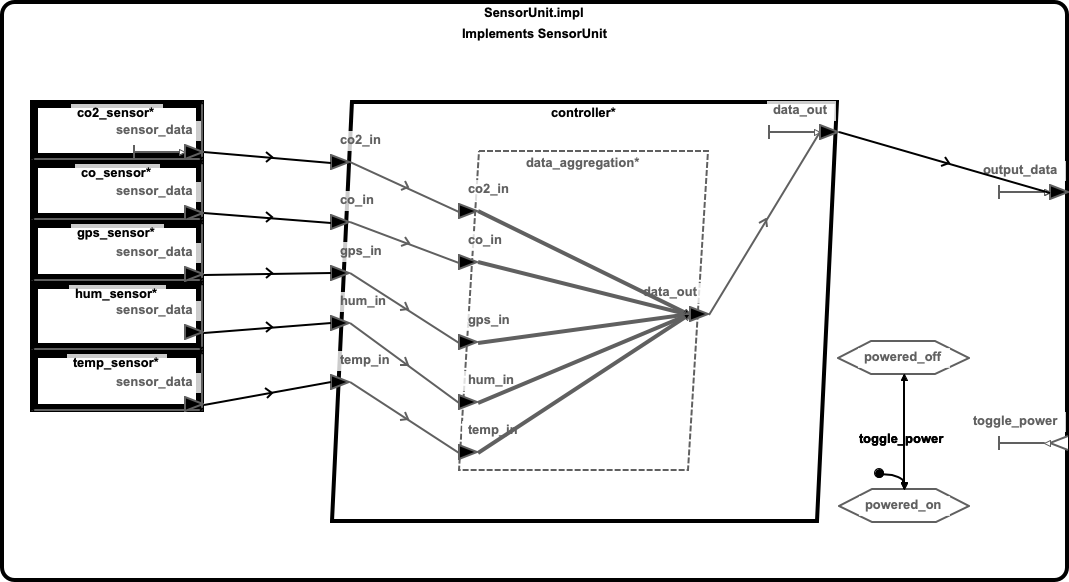
\includegraphics[width=0.9\textwidth]{SensorUnit}
\end{figure*}

\begin{figure*}[h]
\caption{Structure of the Communication Network}
\label{fig:communicationnetwork}
\centering
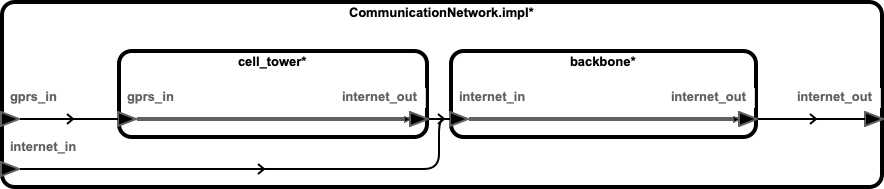
\includegraphics[width=0.9\textwidth]{CommunicationNetwork}
\end{figure*}

\begin{figure}[h]
\caption{Structure of the Control Center}
\label{fig:controlcenter}
\centering
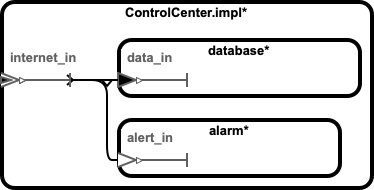
\includegraphics[width=0.45\textwidth]{ControlCenter}
\end{figure}

\subsection{The Sensor Network}

The Sensor Network represents the devices placed within a house or building which together have three purposes: first, collecting environment data that might indicate the presence of a fire; second, sending that data to the Control Center; and third, providing an interface for a local user to monitor the data and configure the sensors. \autoref{fig:sensornetwork} shows the arrangement of the Sensor Network.

To enable this, the Sensor Network is formed by four types of devices:

\begin{enumerate}
	\item Sensor Units, which collect raw environment data;
	\item Communication Units, which receive data from the Sensor Units and forwards it to the relevant destinations;
	\item Mobile Phones, which provide a user interface for monitoring and configuring the other devices; and
	\item one Modem, which connects the Sensor Network to the Internet using wired infrastructure.
\end{enumerate}

The Sensor Units contain five sensors to collect relevant environmental data: ambient temperature, humidity level, carbon monoxide (CO) and dioxide (CO$_2$) concentration, and GPS coordinates.
\autoref{fig:sensorunit} shows the internal structure of a Sensor Unit. 
Since the network can contain multiple Sensor Units (for different rooms inside a house, for example), it is possible to detect precisely where a fire starts and which rooms are affected. 
Sensor Units collect raw environmental data and, using an internal process, combines this information into a single block of data. 
This internal process features a thread that runs at an interval of 100ms to collect and combine data received from sensors.

The combined block of data is then transmitted to the Communication Device using a Zigbee connection. The number of Sensor Units in the network can be configured in a constant value located in `SensorNetwork.aadl`. Furthermore, the Sensor Units have two modes corresponding to their power status. They can be turned on or off when an appropriate signal is received.

Meanwhile, two Communication Devices exist in the network to collect data from the Sensor Units and transmit it elsewhere. The two devices exist for redundancy, so the system can work even if one of them is faulty. There is also an intercommunication port between the two Communication Devices so they work in a synchronized fashion and can avoid duplicated data. Each Communication Device provides ample communication technologies: 
\begin{itemize}
	\item Zigbee to communicate with the Sensor Units;
	\item Bluetooth to communicate with a Mobile Phone;
	\item Wi-fi and Ethernet to connect to a Modem; and
	\item GPRS for cellular communication.
\end{itemize}

Data collected from the Sensor Units is sent over Bluetooth to a Mobile Phone, which allows user interaction. The Wi-fi, Ethernet and GPRS communication techonologies provide both redudancy and flexibility to the system. Ideally, an Ethernet connection provides lower latency communication to the Internet, but Wi-fi and GPRS allow the system to function even if there is a lack of wired infrastructure and permit continuous operation if one is for some reason unavailable.

Aside from providing a bridge between different devices, the Communication Device monitors the sensor data and compares values to a predeterminate threshold. If the temperature, or the CO/CO$_2$ concentration is too high, or the humidity level is too low, an alert signal is sent to the Mobile Phone and to the Control Center, so the necessary measures can be taken.

The Mobile Phone receives data over a Bluetooth connection and displays it in an application. This allows the user to know the current status of the network, the current and historic sensor readings, and control the power each Sensor Unit. Finally, the Modem receives data from the Communication Devices over Wi-fi or Ethernet and transmits packets to the Control Center over the Internet.

The Sensor Network as a whole has two ports to connect to the outside world: one represents a wired connection attached to the Modem, while another shows the cellular GPRS signal sent and received directly by the Communication Device.

\subsection{The Communication Network and the Control Center}

During the development of our model, emphasis was put on the Sensor Network, which we considered the most interesting and complex section of the system. Therefore, the Communication Network and Control Center are rather simple in comparison.

The Communication Network is formed by a Cell Tower, which receives a GPRS signal from the Communication Device and forwards it to the Internet Backbone. The Backbone itself receives wired signal from the Modem or the Cell Tower and abstracts the general Internet infrastructure. \autoref{fig:communicationnetwork} shows the structure of the Communication Network.

The Control Center is the final destination of the sensor readings. It contains a Database, which stores the sensor history for analysis, and an Alarm, which receives an alert signal sent from the Communication Device. With this signal, the designated authorities can dispatch emergency services to the precise location of the fire within a matter of seconds. The Alarm's possible states are modeled as modes: it can either be ringing or not, and switching between modes depends on a signal sent from the Communication Device. \autoref{fig:communicationnetwork} shows the structure of the control center.

\subsection{Auxiliary items}

To help with the structure of the model, a property set and two data types were defined.

The property set allows us to define custom attributes attached to components in the system. 
In it, we defined custom units for data captured by the sensors: temperature is measured in degrees celsius (\degree C), 
humidity is measured in grams per cubic meter (gpm$^3$), 
CO and CO$_2$ concentration is measured in parts per million (ppm) and 
GPS coordinates are tuples of latitude and longitude. 
Each sensor has one or more properties representing the data captured by it.

The data types allow us to analyze the system considering the byte size of data sent through its connections. In our system, each sensor reading can have up to 16 bytes; thus, once the data from the five types of sensors is aggregated and sent through the network, it can be up to 80 bytes of data.

Our analysis is concerned with the connection latency between pairs of components and, therefore, does not suffer influence from the information in the property set and data types.

%\limit{6}

 